%%%%%%%%%%%%%%%%%%%%%%%%%%%%%%%%%%%%%%%%%%%%%%%%%%%%%%%%%%%%%%%%%%%%%%%%%%%
\chapter{Étude de marché}
\label{Chapitre_2}
%%%%%%%%%%%%%%%%%%%%%%%%%%%%%%%%%%%%%%%%%%%%%%%%%%%%%%%%%%%%%%%%%%%%%%%%%%%

\textit{Ce chapitre ne se contente pas de décrire un marché~: il démontre l'existence d'une inefficience opérationnelle structurelle, non adressée, dont Vocallia constitue la réponse directe et défendable. L'analyse croise deux dynamiques complémentaires --- la réalité contrainte du commerce électronique tunisien et la maturité accélérée de l'IA vocale mondiale --- pour établir que l'opportunité est réelle, temporellement bornée et accessible à un premier entrant bien positionné. La méthodologie est pluridisciplinaire~: analyse PESTEL, forces de Porter, cadre TAM/SAM/SOM, étude exploratoire terrain, benchmark concurrentiel et cartographie des parties prenantes. Chaque couche analytique converge vers une même conclusion~: Vocallia répond à un besoin non optionnel, sur un marché captif, dans un horizon d'exécution qui ne restera pas ouvert indéfiniment.}

%%%%%%%%%%%%%%%%%%%%%%%%%%%%%%%%%%%%%%%%%%%%%%%%%%%%%%%%%%%%%%%%%%%%%%%%%%%
\section{Analyse macro-environnementale --- Cadre PESTEL}
\label{section2.1}
%%%%%%%%%%%%%%%%%%%%%%%%%%%%%%%%%%%%%%%%%%%%%%%%%%%%%%%%%%%%%%%%%%%%%%%%%%%

L'analyse PESTEL révèle un alignement remarquable de signaux favorables à l'émergence de Vocallia. Chaque dimension examinée --- politique, économique, sociale, technologique, écologique et légale --- renforce la même conclusion~: les conditions de fond sont réunies et le moment d'entrée sur le marché est optimal.

%%%%%%%%%%%%%%%%%%%%%%%%%%%%%%%%%%%%%%%%%%%%%%%%%%%%%%%%%%%%%%%%%%%%%%%%%%%
\subsection{Environnement politique et légal}
\label{section2.1.1}
%%%%%%%%%%%%%%%%%%%%%%%%%%%%%%%%%%%%%%%%%%%%%%%%%%%%%%%%%%%%%%%%%%%%%%%%%%%

Le Startup Act (Loi n\degre{}2018-20) offre aux structures labellisées des avantages concrets et immédiatement mobilisables~: subventions mensuelles jusqu'à 5\,000~dinars, congé entrepreneurial, exonérations fiscales pluriannuelles et accès facilité à des comptes en devises technologiques. Ce dispositif réduit directement le coût d'amorçage et améliore la compétitivité tarifaire dès le lancement.

Sur le plan réglementaire, la loi n\degre{}2004-63 sur la protection des données personnelles encadre le traitement des enregistrements vocaux. Vocallia intègre cette contrainte dès la conception (\emph{compliance by design})~: consentement explicite en début d'appel, rétention des données limitée à 30~jours, démarche de validation auprès de l'INPDP prévue avant tout déploiement commercial. La loi n\degre{}2000-83 sur le commerce électronique renforce par ailleurs la légitimité des services B2B numériques.

Ce cadre réglementaire, loin de constituer un simple coût de gestion, fonctionne en réalité comme une barrière à l'entrée au bénéfice de Vocallia. Toute solution internationale souhaitant pénétrer le marché tunisien devra investir dans une mise en conformité locale spécifique, sans bénéficier du Startup Act ni de la crédibilité institutionnelle que Vocallia construit dès l'origine. La rigueur réglementaire adoptée \emph{ab initio} crée ainsi un avantage compétitif défendable vis-à-vis des acteurs globaux, tout en réduisant le risque juridique perçu par les marchands partenaires --- accélérant de facto l'adoption commerciale.

%%%%%%%%%%%%%%%%%%%%%%%%%%%%%%%%%%%%%%%%%%%%%%%%%%%%%%%%%%%%%%%%%%%%%%%%%%%
\subsection{Environnement économique}
\label{section2.1.2}
%%%%%%%%%%%%%%%%%%%%%%%%%%%%%%%%%%%%%%%%%%%%%%%%%%%%%%%%%%%%%%%%%%%%%%%%%%%

Le e-commerce tunisien affiche une dynamique de croissance soutenue et durable~: 1\,126 sites marchands actifs en 2024, un volume de transactions de 1\,241,2~millions de dinars (BCT, 2024), et une progression de 41,6~\% du chiffre d'affaires entre juin 2022 et juin 2023, à 538,8~millions de dinars. Cette croissance n'est pas cyclique~: elle traduit une adoption progressive et durable des comportements d'achat numériques.

Mais le fait économique le plus structurant pour Vocallia est celui-ci~: \textbf{84~\% des transactions e-commerce tunisiennes sont réglées en espèces à la livraison (\emph{cash on delivery}).} Cette réalité rend la confirmation téléphonique préalable à l'expédition quasi-systématique --- et non optionnelle. Chaque commande expédiée sans confirmation expose le marchand à un retour non anticipé~: frais de transport aller-retour, manutention, réemballage et immobilisation temporaire du stock. En ordre de grandeur, le coût unitaire d'un colis retourné se situe entre 4 et 8~DT selon la catégorie de produit et la zone géographique de livraison.

Pour un e-commerçant de petite taille traitant 10 à 15 commandes par jour --- profil représentatif de la majorité des marchands tunisiens --- avec un taux de retour de l'ordre de 20 à 30~\%, la perte mensuelle liée aux livraisons échouées peut être estimée entre \textbf{300 et 700~DT}. À cela s'ajoute le coût de la main-d'\oe uvre affectée aux appels de confirmation~: qu'il s'agisse du gérant lui-même ou d'un employé dédié, ce poste représente entre 400 et 700~DT par mois --- pour une tâche répétitive, chronophage et parfaitement automatisable. Ces estimations restent des ordres de grandeur prudents~; elles suffisent néanmoins à établir que le problème n'est pas marginal~: même dans l'hypothèse basse, le coût cumulé des retours et de la gestion manuelle représente une charge mensuelle de 700 à 1\,400~DT --- significative pour une PME dont les marges opérationnelles sont étroites, et suffisante pour justifier économiquement le recours à une solution d'automatisation.

Le constat est arithmétique~: à mesure que le volume de commandes croît, la confirmation manuelle devient non scalable --- chaque palier de croissance impose un recrutement supplémentaire que les marges du secteur ne peuvent absorber. L'automatisation n'est plus une option d'optimisation~: elle devient une condition de survie opérationnelle.

\begin{figure}[H]
    \centering
    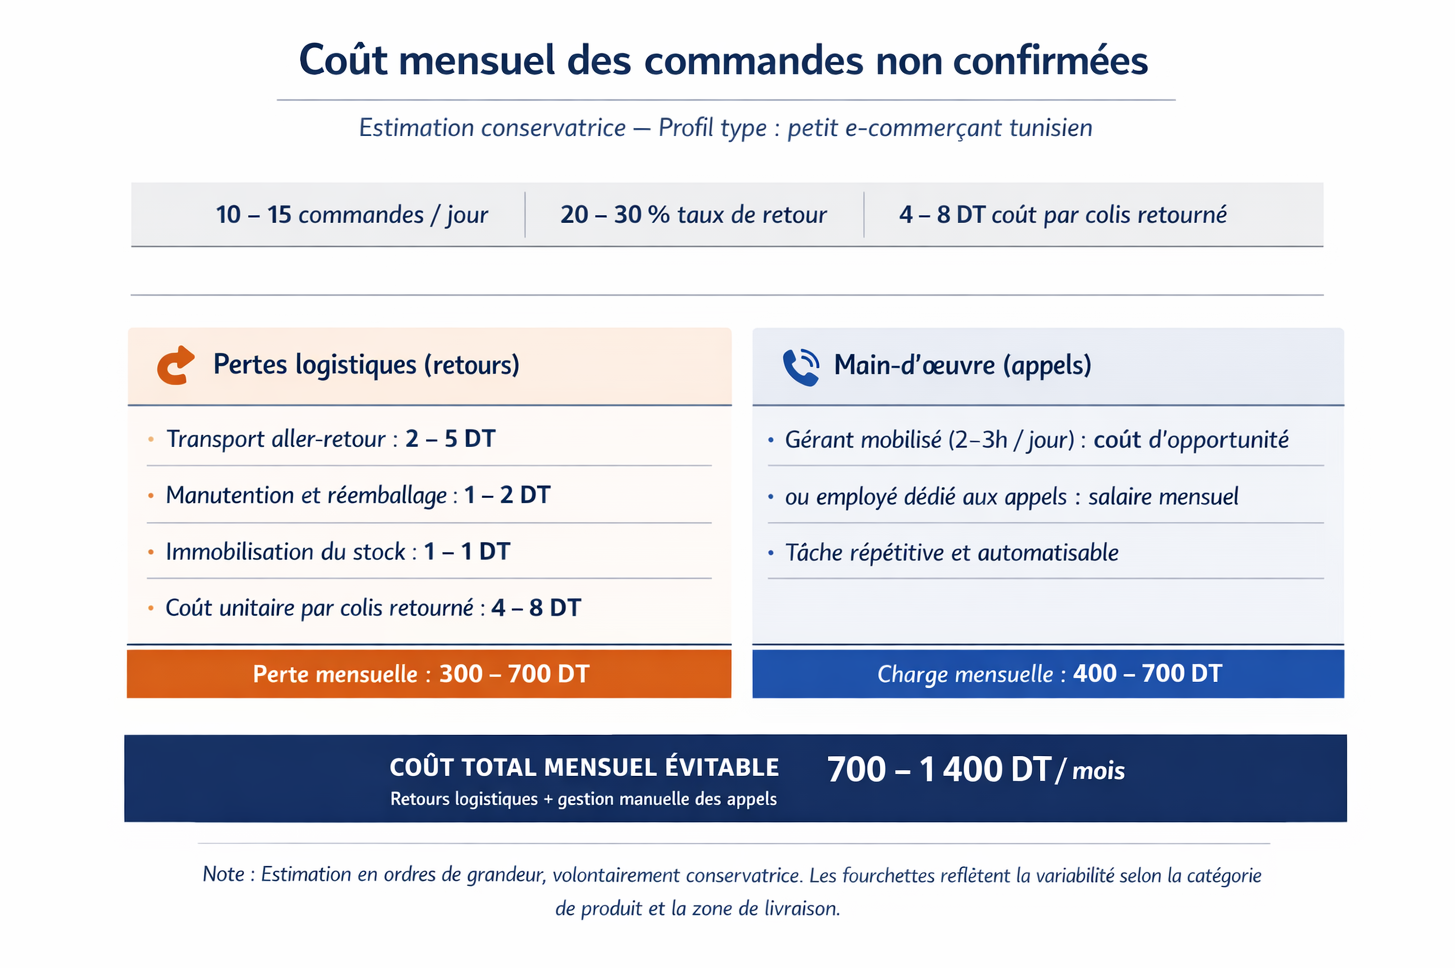
\includegraphics[width=0.92\textwidth]{figures/cout-commande-non-confirmee.png}
    \caption{Estimation du coût mensuel des commandes non confirmées --- Profil type d'un petit e-commerçant tunisien}
    \label{fig:cout-commande-non-confirmee}
\end{figure}

Le \emph{cash on delivery} n'est pas une anomalie appelée à disparaître~: il est ancré dans la méfiance du consommateur tunisien envers le paiement en ligne et dans l'absence d'infrastructure de confiance numérique généralisée. Tant que cette réalité persiste --- horizon incertain à moyen terme --- la confirmation téléphonique reste obligatoire, et donc automatisable. Plus décisif encore~: la croissance de 41,6~\% du secteur amplifie mécaniquement ce besoin, puisque chaque nouvelle commande génère un appel de confirmation supplémentaire. Le marché adressable de Vocallia croît ainsi sans effort commercial additionnel.

\textit{Source~: BCT, Bulletin sur les paiements en chiffres en Tunisie, exercice 2024 (mars 2025)~; BCT, Rapport sur les paiements 2022-2023~; estimation Vocallia sur la base des variables terrain, 2025.}

%%%%%%%%%%%%%%%%%%%%%%%%%%%%%%%%%%%%%%%%%%%%%%%%%%%%%%%%%%%%%%%%%%%%%%%%%%%
\subsection{Environnement social et démographique}
\label{section2.1.3}
%%%%%%%%%%%%%%%%%%%%%%%%%%%%%%%%%%%%%%%%%%%%%%%%%%%%%%%%%%%%%%%%%%%%%%%%%%%

La Tunisie compte 12,3~millions d'habitants en 2024, avec un taux de pénétration d'Internet de 66~\% (INS, 2022). Selon le baromètre MDWEB (vague~4, 2023), 75~\% des internautes ont déjà acheté en ligne, dont plus de la moitié au moins une fois par mois. Cette base d'acheteurs croissante alimente mécaniquement le volume de commandes des marchands, et donc le nombre d'appels de confirmation à passer. Il existe un seuil --- généralement situé autour de 50 à 80 commandes quotidiennes --- au-delà duquel la gestion manuelle des appels cesse d'être un choix organisationnel et devient un goulet d'étranglement~: le marchand ne peut plus croître sans automatiser ou recruter, et les marges du secteur interdisent le second. Le taux de chômage de 16,4~\% (INS, 2024), combiné à une pression à la hausse sur les coûts salariaux, renforce l'attractivité économique de l'automatisation pour des PME dont les marges opérationnelles restent étroites.

La dynamique d'ensemble est celle d'un cercle vicieux, représenté en figure~\ref{fig:cercle-vicieux}~: la croissance du marché génère davantage de commandes, donc davantage d'appels, ce qui sature le gérant, provoque des livraisons échouées, érode les marges et empêche le recrutement --- ramenant le marchand au point de départ. Chaque heure passée au téléphone à confirmer des commandes est une heure non investie dans la croissance --- et dans un marché en expansion de 41,6~\% par an, le coût de cette inaction se compose trimestre après trimestre.

\begin{figure}[H]
    \centering
    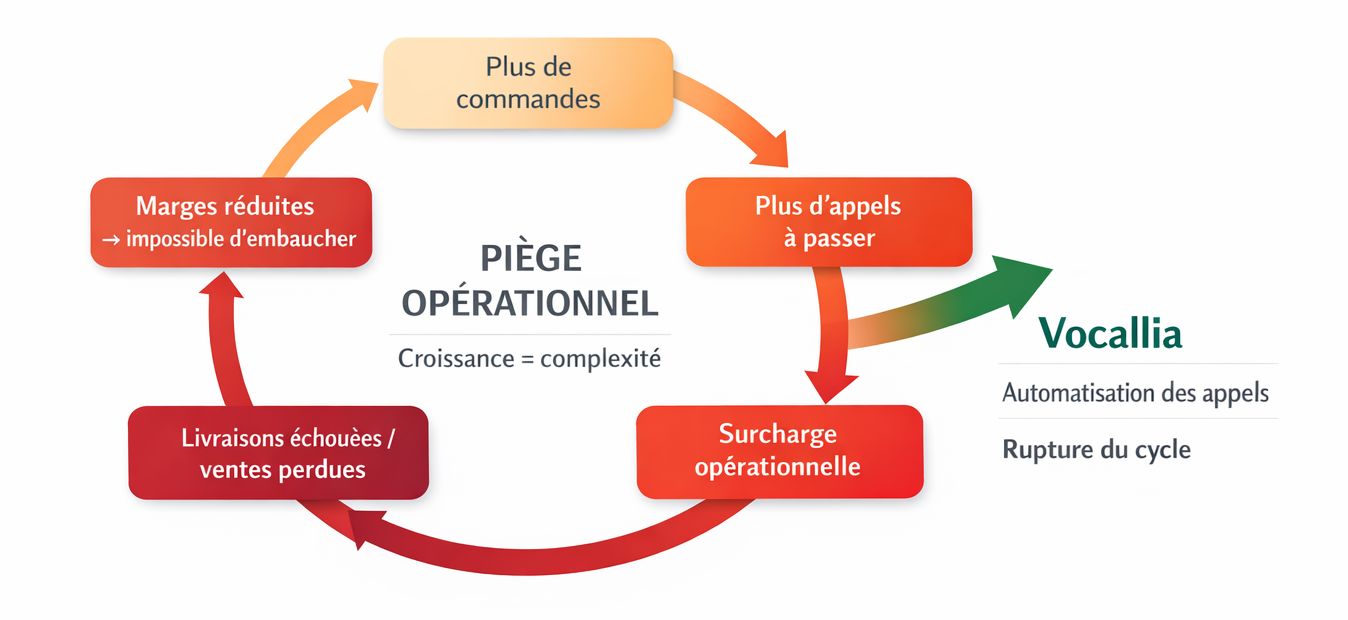
\includegraphics[width=0.78\textwidth]{figures/cercle-vicieux-marchand.png}
    \caption{Le cercle vicieux du marchand e-commerce sans automatisation}
    \label{fig:cercle-vicieux}
\end{figure}

Le positionnement ROI de Vocallia repose sur deux axes complémentaires~: la réduction des coûts directs mesurables (salaire, retours logistiques) et la libération du temps stratégique du dirigeant --- argument décisif dans un segment où la surcharge opérationnelle constitue le principal frein à la croissance.

\textit{Source~: INS, Enquête sur la population et l'emploi, 2024~; MDWEB, Baromètre e-commerce vague~4, 2023.}

%%%%%%%%%%%%%%%%%%%%%%%%%%%%%%%%%%%%%%%%%%%%%%%%%%%%%%%%%%%%%%%%%%%%%%%%%%%
\subsection{Environnement technologique}
\label{section2.1.4}
%%%%%%%%%%%%%%%%%%%%%%%%%%%%%%%%%%%%%%%%%%%%%%%%%%%%%%%%%%%%%%%%%%%%%%%%%%%

Le marché mondial de l'IA conversationnelle atteindra 41,39~milliards de dollars d'ici 2030, depuis 11,58~milliards en 2024 (CAGR de 23,7~\%, Grand View Research, 2024). Le segment des agents vocaux IA croît encore plus vite~: 34,8~\% par an entre 2024 et 2034 (Market.us, 2024), confirmé par Technavio à 37,2~\% sur 2024-2029. Cette dynamique traduit non pas une mode, mais une transition technologique de fond dans la gestion de la relation client.

Cette transition est rendue possible par la conjonction de trois maturités techniques simultanées~: la reconnaissance vocale (STT), portée notamment par Whisper d'OpenAI --- avec des limites persistantes sur le darija qui constituent précisément la niche de Vocallia~; les modèles de langage (LLM) accessibles via API à coût décroissant~; et la synthèse vocale (TTS), dont la naturalité progresse rapidement. Les contraintes techniques résiduelles --- latence cible inférieure à 800~ms, gestion des hallucinations sur cas-limites --- sont gérées par une architecture de \emph{fallback} vers un agent humain et par un périmètre fonctionnel volontairement restreint au lancement.

Vocallia entre sur le marché au moment précis où la technologie vocale IA est suffisamment mature pour être viable, et suffisamment récente pour que le marché local soit encore vierge --- ce qui constitue la définition même d'un point d'entrée optimal. Dans 18 à 24~mois, cet avantage temporel se réduira~: soit les API globales progresseront significativement sur l'arabe dialectal, soit des concurrents locaux auront émergé. Chaque mois d'avance se traduit en données propriétaires accumulées, en clients intégrés et en réputation marché --- trois actifs que nul entrant futur ne pourra racheter. L'urgence d'exécution n'est donc pas tactique~: elle est technologiquement et concurrentiellement fondée.

\textit{Source~: Grand View Research, Conversational AI Market Report, 2024~; Market.us, Voice AI Agents Market, 2024~; Technavio, Voice AI Agents Market Forecast 2025-2029.}

%%%%%%%%%%%%%%%%%%%%%%%%%%%%%%%%%%%%%%%%%%%%%%%%%%%%%%%%%%%%%%%%%%%%%%%%%%%
\subsection{Environnement écologique}
\label{section2.1.5}
%%%%%%%%%%%%%%%%%%%%%%%%%%%%%%%%%%%%%%%%%%%%%%%%%%%%%%%%%%%%%%%%%%%%%%%%%%%

Le modèle opérationnel de Vocallia génère un bilan environnemental indirect favorable~: en réduisant les expéditions non confirmées, la solution diminue les émissions logistiques liées aux retours. Le recours à une infrastructure cloud mutualisée produit une empreinte carbone par interaction nettement inférieure à celle d'un centre d'appels physique. À terme, un déploiement sur serveurs locaux (OVH Tunisie ou infrastructure privée) est envisagé pour les secteurs sensibles, renforçant simultanément la souveraineté des données et la maîtrise de l'empreinte numérique. Cet impact environnemental positif constitue par ailleurs un levier d'éligibilité aux programmes de financement à dimension ESG --- critère d'accès croissant aux appels à projets institutionnels et aux fonds d'investissement à impact.

%%%%%%%%%%%%%%%%%%%%%%%%%%%%%%%%%%%%%%%%%%%%%%%%%%%%%%%%%%%%%%%%%%%%%%%%%%%
\subsection{Environnement légal --- Éthique de l'IA vocale et protection des données}
\label{section2.1.6}
%%%%%%%%%%%%%%%%%%%%%%%%%%%%%%%%%%%%%%%%%%%%%%%%%%%%%%%%%%%%%%%%%%%%%%%%%%%

Vocallia opère dans un espace réglementaire en cours de structuration. Trois principes éthiques et légaux sont intégrés dès la conception du produit, sans compromis. \textbf{Premièrement}, le consentement explicite~: chaque appel s'ouvre par une annonce claire de sa nature automatisée, conformément à la loi n\degre{}2004-63 --- protection simultanée du client final et du marchand contre tout risque de contentieux. \textbf{Deuxièmement}, la minimisation des données~: conservation des enregistrements vocaux et transcriptions limitée à 30~jours par défaut, avec suppression sur demande. \textbf{Troisièmement}, le droit au transfert humain~: chaque scénario d'appel intègre un mécanisme de redirection vers un agent humain dès que la requête dépasse les capacités du système, garantissant la qualité de l'expérience sans risque de blocage.

À mesure que les régulations autour de l'IA vocale se durciront --- tendance mondiale irréversible --- les acteurs n'ayant pas intégré ces exigences dès l'origine subiront des coûts de mise en conformité élevés et des délais d'adaptation. Vocallia, ayant construit sa conformité comme fondation opérationnelle et non comme ajout tardif, transforme chaque renforcement réglementaire futur en avantage concurrentiel supplémentaire vis-à-vis des entrants moins rigoureux.

\begin{figure}[H]
    \centering
    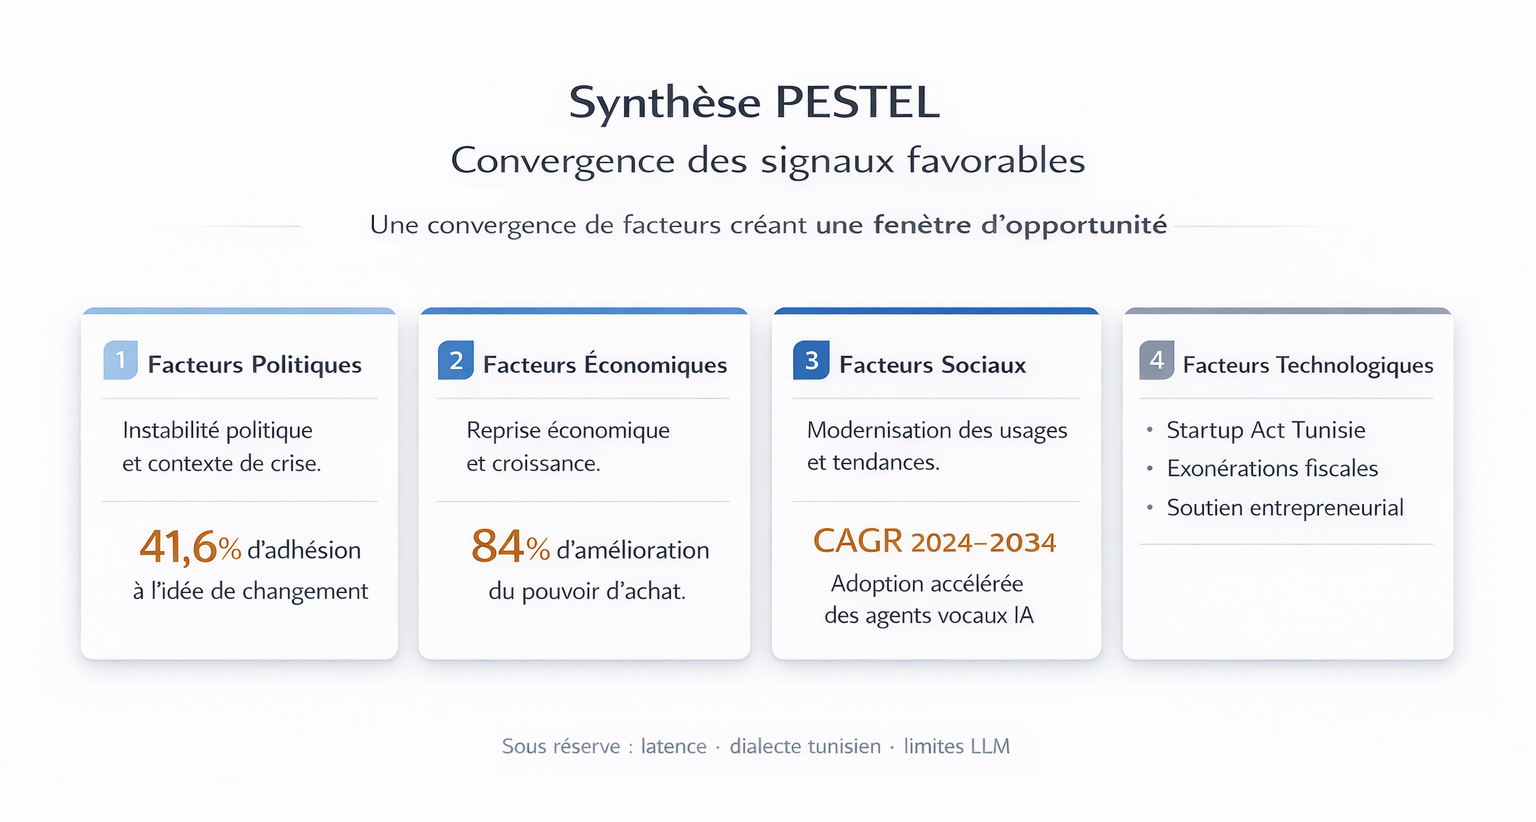
\includegraphics[width=0.95\textwidth]{figures/pestel-convergences.png}
    \caption{Synthèse PESTEL~: convergence des signaux favorables pour Vocallia}
    \label{fig:pestel-convergences}
\end{figure}

L'environnement macro étant caractérisé, il convient d'examiner la dynamique concurrentielle du secteur lui-même --- c'est l'objet de l'analyse sectorielle qui suit.

%%%%%%%%%%%%%%%%%%%%%%%%%%%%%%%%%%%%%%%%%%%%%%%%%%%%%%%%%%%%%%%%%%%%%%%%%%%
\section{Analyse sectorielle --- Les cinq forces de Porter}
\label{section2.2}
%%%%%%%%%%%%%%%%%%%%%%%%%%%%%%%%%%%%%%%%%%%%%%%%%%%%%%%%%%%%%%%%%%%%%%%%%%%

Appliqué au marché de l'automatisation vocale B2B en Tunisie, le modèle de Porter (1979) révèle un secteur fondamentalement attractif à court terme, dont les vulnérabilités sont identifiées, gérées et en partie transformées en leviers stratégiques par Vocallia. La figure~\ref{fig:porter-five-forces} synthétise le niveau de chaque force~; les sous-sections qui suivent en détaillent les mécanismes.

\begin{figure}[H]
    \centering
    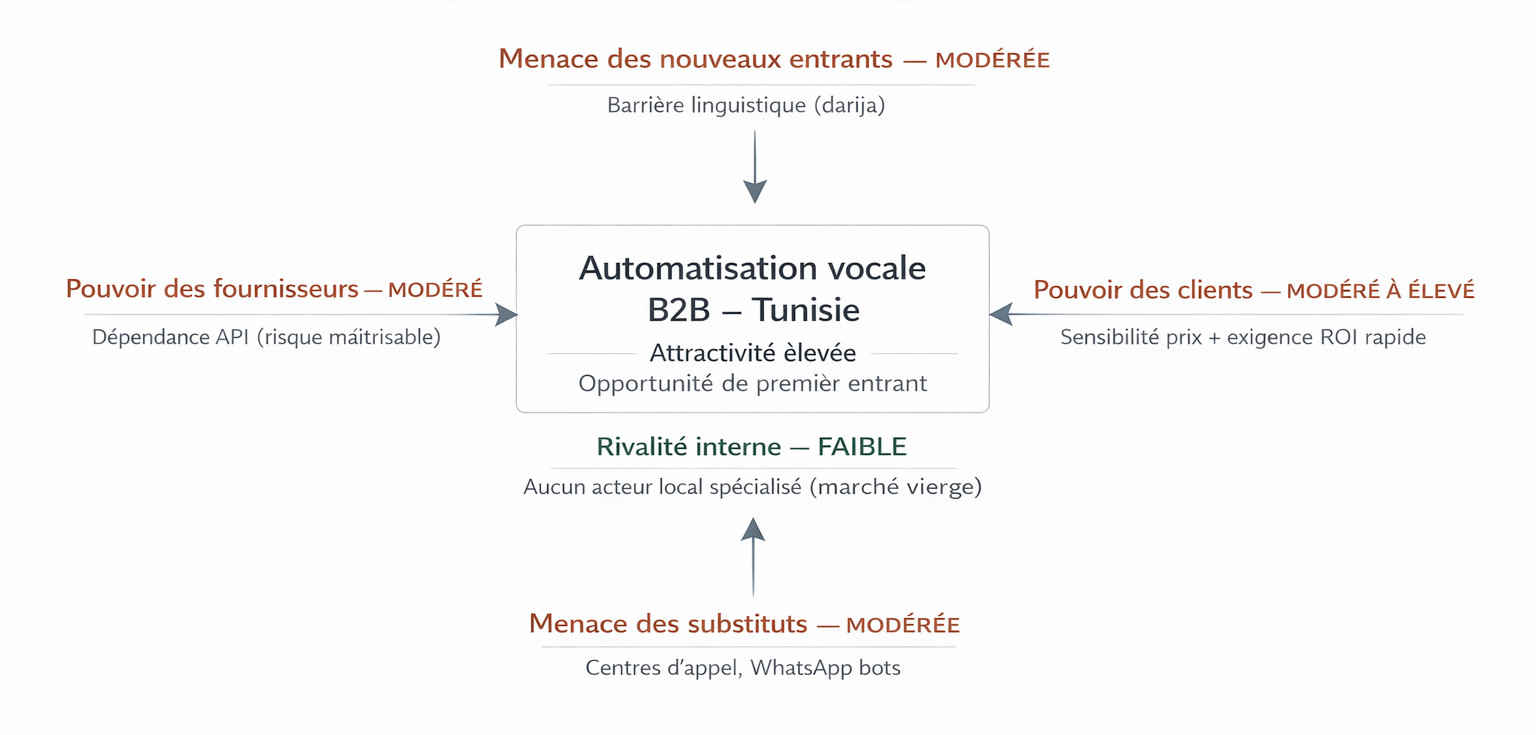
\includegraphics[width=0.82\textwidth]{figures/porter-five-forces-vocallia.png}
    \caption{Synthèse des cinq forces de Porter --- Marché de l'automatisation vocale B2B en Tunisie}
    \label{fig:porter-five-forces}
\end{figure}

%%%%%%%%%%%%%%%%%%%%%%%%%%%%%%%%%%%%%%%%%%%%%%%%%%%%%%%%%%%%%%%%%%%%%%%%%%%
\subsection{Force 1 --- Rivalité interne (faible)}
\label{section2.2.1}
%%%%%%%%%%%%%%%%%%%%%%%%%%%%%%%%%%%%%%%%%%%%%%%%%%%%%%%%%%%%%%%%%%%%%%%%%%%

Aucun acteur local ne propose aujourd'hui de solution d'agent vocal IA spécialisée pour les e-commerçants tunisiens. La rivalité directe est nulle. Cette situation crée une opportunité de premier entrant dont la valeur est inversement proportionnelle à sa durée~: dans un horizon de 18 à 36~mois, si Vocallia démontre la viabilité du modèle, des concurrents locaux ou des solutions internationales adaptées émergeront. La stratégie de défense est claire~: convertir cette avance temporelle en actifs durables --- base clients active, corpus de données propriétaires, réputation marché. Le premier acteur à atteindre la masse critique crédentielle --- 30 à 50~clients actifs, plusieurs dizaines de milliers d'appels traités, intégrations déployées --- s'imposera comme standard de référence et bénéficiera d'un effet réseau de réputation que la concurrence ne pourra dupliquer qu'au prix d'un investissement considérable.

%%%%%%%%%%%%%%%%%%%%%%%%%%%%%%%%%%%%%%%%%%%%%%%%%%%%%%%%%%%%%%%%%%%%%%%%%%%
\subsection{Force 2 --- Menace des nouveaux entrants (modérée)}
\label{section2.2.2}
%%%%%%%%%%%%%%%%%%%%%%%%%%%%%%%%%%%%%%%%%%%%%%%%%%%%%%%%%%%%%%%%%%%%%%%%%%%

Les barrières à l'entrée sont réelles mais non permanentes. La plus significative est linguistique~: la maîtrise du darija --- dialecte non standardisé, caractérisé par un code-switching arabe/français dense et une variabilité phonologique régionale --- exige des données d'entraînement locales spécifiques qu'aucun acteur global ne possède. Le risque principal est la désintermédiation technologique~: si des fournisseurs globaux comme OpenAI améliorent leur couverture de l'arabe dialectal, la barrière linguistique s'érode partiellement. Ce risque est contenu par l'accumulation active d'un corpus propriétaire de données vocales en darija --- actif immatériel non reproductible sans historique opérationnel local.

La barrière linguistique constitue ainsi le point de départ, non le point d'arrivée de la défendabilité de Vocallia. Sa pérennité dépend de la capacité à la transformer en un fossé de données auto-entretenu, dont le mécanisme de \emph{flywheel} est détaillé en figure~\ref{fig:flywheel-vocallia}. L'apprentissage continu produit un effet de composition~: chaque itération du modèle améliore la capacité du système à extraire de la valeur des données futures, créant un écart de performance qui s'accélère plutôt qu'il ne se stabilise. Un concurrent entrant dans 24~mois ne pourra pas acheter cet historique --- il devra le reconstruire entièrement, avec les erreurs et le temps que cela implique.

%%%%%%%%%%%%%%%%%%%%%%%%%%%%%%%%%%%%%%%%%%%%%%%%%%%%%%%%%%%%%%%%%%%%%%%%%%%
\subsection{Force 3 --- Pouvoir de négociation des clients (modéré à élevé)}
\label{section2.2.3}
%%%%%%%%%%%%%%%%%%%%%%%%%%%%%%%%%%%%%%%%%%%%%%%%%%%%%%%%%%%%%%%%%%%%%%%%%%%

Les e-commerçants tunisiens sont des PME à forte sensibilité prix et à exigence de ROI rapide. Ce pouvoir de négociation est toutefois limité par l'absence d'alternative directe~: sans concurrent comparable, le client ne peut pas «~faire jouer la concurrence~». La stratégie d'entrée de Vocallia --- pilote à faible engagement initial --- réduit le risque perçu et abaisse la friction à l'adoption. Une fois l'intégration technique déployée (connexion API, scripts personnalisés, synchronisation des commandes), les coûts de changement deviennent significatifs~: migrer vers une solution concurrente implique de tout recommencer --- formation, paramétrage, historique des appels, personnalisation des flux. Ces \emph{switching costs} ne sont pas statiques~: ils s'accroissent avec la durée de la relation, à mesure que l'historique d'appels et les données de performance accumulées deviennent des actifs opérationnels dont le client dépend quotidiennement.

%%%%%%%%%%%%%%%%%%%%%%%%%%%%%%%%%%%%%%%%%%%%%%%%%%%%%%%%%%%%%%%%%%%%%%%%%%%
\subsection{Force 4 --- Pouvoir de négociation des fournisseurs (modéré)}
\label{section2.2.4}
%%%%%%%%%%%%%%%%%%%%%%%%%%%%%%%%%%%%%%%%%%%%%%%%%%%%%%%%%%%%%%%%%%%%%%%%%%%

Vocallia dépend de fournisseurs d'API globaux (OpenAI, ElevenLabs, Twilio) dont les tarifs sont standardisés et peu négociables en phase d'amorçage. Ce risque est contenu par une architecture multi-fournisseurs permettant la substitution rapide en cas de hausse tarifaire ou d'interruption de service. À mesure que le volume d'appels croît, les économies d'échelle sur les API réduisent le coût par appel et élargissent les marges opérationnelles. La dépendance fournisseurs est donc une contrainte d'amorçage, gérée par \emph{design}, qui se renverse avec la croissance~: le \emph{scaling} du volume transforme Vocallia en client significatif pour ses \emph{providers}, ouvrant des conditions préférentielles et améliorant durablement les marges.

%%%%%%%%%%%%%%%%%%%%%%%%%%%%%%%%%%%%%%%%%%%%%%%%%%%%%%%%%%%%%%%%%%%%%%%%%%%
\subsection{Force 5 --- Menace des substituts (modérée)}
\label{section2.2.5}
%%%%%%%%%%%%%%%%%%%%%%%%%%%%%%%%%%%%%%%%%%%%%%%%%%%%%%%%%%%%%%%%%%%%%%%%%%%

Trois catégories de substituts sont identifiables~: les agents humains internes (coût élevé, scalabilité nulle), les centres d'appels externalisés (coût variable élevé, perte de contrôle relationnel), et les chatbots textuels WhatsApp/Messenger (déploiement facile, mais canal non équivalent au vocal pour la confirmation de commandes). Aucun ne combine scalabilité illimitée, disponibilité 24h/24, coût faible par interaction et conversation vocale en dialecte tunisien. Les chatbots WhatsApp Business constituent la menace la plus crédible à court terme, mais leur limite est structurelle~: le canal textuel génère des taux de réponse et de conversion inférieurs au vocal, où la voix --- même synthétisée --- crée un niveau d'engagement que le texte ne peut reproduire. Vocallia devra démontrer cette supériorité par des données chiffrées lors de la phase pilote.

\begin{tcolorbox}[colback=gray!8, colframe=gray!50, title=\textbf{Attractivité sectorielle --- Verdict Porter}, fonttitle=\bfseries]
\textbf{Le secteur est fondamentalement attractif aujourd'hui, et cette attractivité est temporaire.} Rivalité directe nulle, barrière linguistique défendable, substituts incomplets~: les conditions d'entrée sont exceptionnellement favorables. Les deux risques à surveiller --- désintermédiation technologique et émergence de nouveaux entrants capitalisés --- partagent la même réponse stratégique~: l'accumulation accélérée de données propriétaires et de clients actifs. Chaque jour d'opération construit une position que nul entrant futur ne pourra reprendre sans investir plusieurs fois la mise initiale de Vocallia.
\end{tcolorbox}

L'attractivité sectorielle étant établie, la question suivante est celle de la taille du marché capturable --- et de la trajectoire commerciale réaliste à trois ans.

%%%%%%%%%%%%%%%%%%%%%%%%%%%%%%%%%%%%%%%%%%%%%%%%%%%%%%%%%%%%%%%%%%%%%%%%%%%
\section{Quantification du marché cible --- Cadre TAM / SAM / SOM}
\label{section2.3}
%%%%%%%%%%%%%%%%%%%%%%%%%%%%%%%%%%%%%%%%%%%%%%%%%%%%%%%%%%%%%%%%%%%%%%%%%%%

Le cadre TAM/SAM/SOM permet de distinguer le potentiel théorique d'un marché de la cible commerciale réaliste à court terme. Les estimations ci-après reposent sur les données officielles de la BCT (2024) et les résultats de l'étude exploratoire Muvaka (avril 2025). Elles sont volontairement conservatrices~: elles excluent le commerce informel via réseaux sociaux et l'extension à d'autres secteurs, qui constituent des vecteurs d'\emph{upside} non intégrés dans les projections de base.

%%%%%%%%%%%%%%%%%%%%%%%%%%%%%%%%%%%%%%%%%%%%%%%%%%%%%%%%%%%%%%%%%%%%%%%%%%%
\subsection{TAM --- Marché total adressable}
\label{section2.3.1}
%%%%%%%%%%%%%%%%%%%%%%%%%%%%%%%%%%%%%%%%%%%%%%%%%%%%%%%%%%%%%%%%%%%%%%%%%%%

Le TAM de Vocallia recouvre l'ensemble des entités tunisiennes ayant un besoin régulier et récurrent d'appels clients sortants. La BCT recensait 1\,126 sites marchands actifs en 2024. Le baromètre MDWEB (vague~4, 2023) suggère que le volume des transactions informelles via réseaux sociaux serait d'une ampleur comparable au marché formel --- hypothèse cohérente avec la structure duale du commerce tunisien. En intégrant les e-commerçants informels, les agences, cabinets médicaux, services de livraison et centres de formation, le TAM est estimé à \textbf{plus de 8\,000 entités potentielles}. L'architecture modulaire de la solution --- scripts paramétrables par secteur --- permet d'adresser ces verticaux sans refonte technologique majeure, transformant le TAM d'une estimation statique en un marché expansible par \emph{design}.

\textit{Source~: BCT, Bulletin sur les paiements 2024~; MDWEB, Baromètre e-commerce vague~4, 2023.}

%%%%%%%%%%%%%%%%%%%%%%%%%%%%%%%%%%%%%%%%%%%%%%%%%%%%%%%%%%%%%%%%%%%%%%%%%%%
\subsection{SAM --- Marché serviceable}
\label{section2.3.2}
%%%%%%%%%%%%%%%%%%%%%%%%%%%%%%%%%%%%%%%%%%%%%%%%%%%%%%%%%%%%%%%%%%%%%%%%%%%

Le SAM est délimité aux e-commerçants dont la volumétrie d'appels justifie économiquement le recours à une solution SaaS B2B, et dont la structure organisationnelle est suffisamment formalisée pour l'adopter. Les données Muvaka (22 répondants, avril 2025) indiquent que 63,7~\% des répondants traitent plus de 5 appels de confirmation par jour --- seuil à partir duquel l'automatisation devient rentable dès le premier mois. En extrapolant prudemment à la base officielle de 1\,126 marchands actifs (BCT 2024), le SAM est estimé entre \textbf{700 et 900 e-commerçants}. Ce chiffre sous-estime vraisemblablement le marché réel, dans la mesure où il exclut l'ensemble du commerce informel.

%%%%%%%%%%%%%%%%%%%%%%%%%%%%%%%%%%%%%%%%%%%%%%%%%%%%%%%%%%%%%%%%%%%%%%%%%%%
\subsection{SOM --- Marché capturable à 3 ans}
\label{section2.3.3}
%%%%%%%%%%%%%%%%%%%%%%%%%%%%%%%%%%%%%%%%%%%%%%%%%%%%%%%%%%%%%%%%%%%%%%%%%%%

Le SOM représente la cible commerciale réaliste à trois ans. L'objectif est de capter entre 5 et 8~\% du SAM, soit \textbf{40 à 70 clients actifs en fin d'année~3}. À un revenu mensuel récurrent moyen de 120~DT par client, le SOM se traduit par un chiffre d'affaires annuel récurrent cible entre \textbf{57\,600~DT et 100\,800~DT} --- avant toute extension sectorielle.

Ces projections sont délibérément prudentes~: elles reposent sur un rythme d'acquisition de 1 à 2 nouveaux clients par mois, sans croissance organique par recommandation. Le SOM projeté représente la borne basse crédible d'un scénario sans levier externe, et constitue le socle à partir duquel chaque extension sectorielle --- santé, immobilier, logistique, formation --- représente un multiplicateur de revenus sans coût marginal élevé. À horizon cinq ans, la confirmation de commandes constitue le cas d'usage d'ancrage --- le point d'entrée à partir duquel Vocallia a vocation à devenir une infrastructure conversationnelle complète~: relance de paniers abandonnés, enquêtes de satisfaction, prise de rendez-vous médicaux, qualification de leads immobiliers. Chaque vertical ajouté réutilise le même socle technologique, le même corpus linguistique et la même base de clients, transformant un outil mono-usage en plateforme à revenus composés.

\begin{figure}[H]
    \centering
    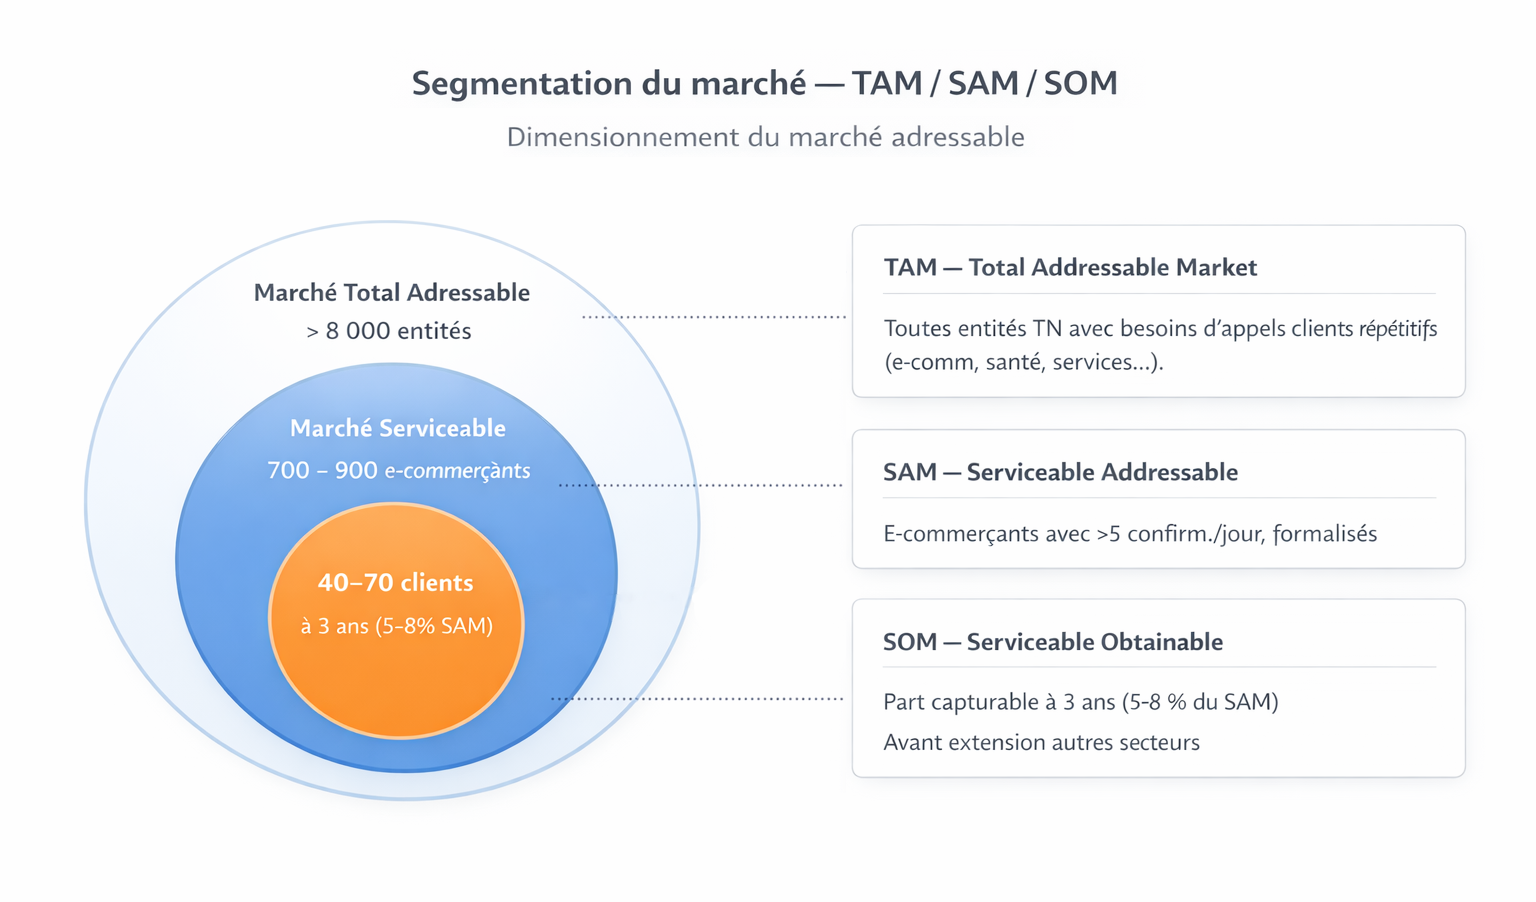
\includegraphics[width=\textwidth]{figures/tam-sam-som-vocallia.png}
    \caption{Représentation visuelle du TAM, SAM et SOM de Vocallia (2025)}
    \label{fig:tam-sam-som-vocallia}
\end{figure}

Les estimations quantitatives qui précèdent reposent sur des données secondaires. Pour les confronter à la réalité du terrain, une étude exploratoire a été conduite directement auprès des e-commerçants.

%%%%%%%%%%%%%%%%%%%%%%%%%%%%%%%%%%%%%%%%%%%%%%%%%%%%%%%%%%%%%%%%%%%%%%%%%%%
\section{Étude exploratoire terrain --- Phase Muvaka (avril 2025)}
\label{section2.4}
%%%%%%%%%%%%%%%%%%%%%%%%%%%%%%%%%%%%%%%%%%%%%%%%%%%%%%%%%%%%%%%%%%%%%%%%%%%

Avant de figer l'identité commerciale sous le nom Vocallia, une phase d'exploration de marché a été conduite en avril 2025 sous la marque de test Muvaka. Ce choix méthodologique, inspiré des pratiques du \emph{Lean Startup} (Ries, 2011), visait à tester la réceptivité du marché sans biais d'identité de marque, et à recueillir des données primaires directement auprès des e-commerçants tunisiens dans leur réalité opérationnelle.

Avec 22 répondants, les résultats constituent une étude exploratoire qualitative, non une validation statistique généralisable. Leur valeur réside dans la cohérence interne des signaux observés et leur convergence avec les données macroéconomiques établies dans les sections précédentes.

%%%%%%%%%%%%%%%%%%%%%%%%%%%%%%%%%%%%%%%%%%%%%%%%%%%%%%%%%%%%%%%%%%%%%%%%%%%
\subsection{Dispositif de collecte}
\label{section2.4.1}
%%%%%%%%%%%%%%%%%%%%%%%%%%%%%%%%%%%%%%%%%%%%%%%%%%%%%%%%%%%%%%%%%%%%%%%%%%%

Le dispositif combinait une \emph{landing page} de capture d'intérêt, un formulaire structuré de 9 questions et deux campagnes Meta Ads (Facebook / Instagram) complémentaires, déployées sur 7 jours avec un budget total de 20~euros --- démarche de validation à coût marginal, cohérente avec le stade d'amorçage.

%%%%%%%%%%%%%%%%%%%%%%%%%%%%%%%%%%%%%%%%%%%%%%%%%%%%%%%%%%%%%%%%%%%%%%%%%%%
\subsection{Résultats des campagnes Meta Ads}
\label{section2.4.2}
%%%%%%%%%%%%%%%%%%%%%%%%%%%%%%%%%%%%%%%%%%%%%%%%%%%%%%%%%%%%%%%%%%%%%%%%%%%

Deux campagnes aux objectifs complémentaires ont mesuré à la fois l'attractivité du message et la capacité à générer des leads qualifiés.

\begin{figure}[H]
    \centering
    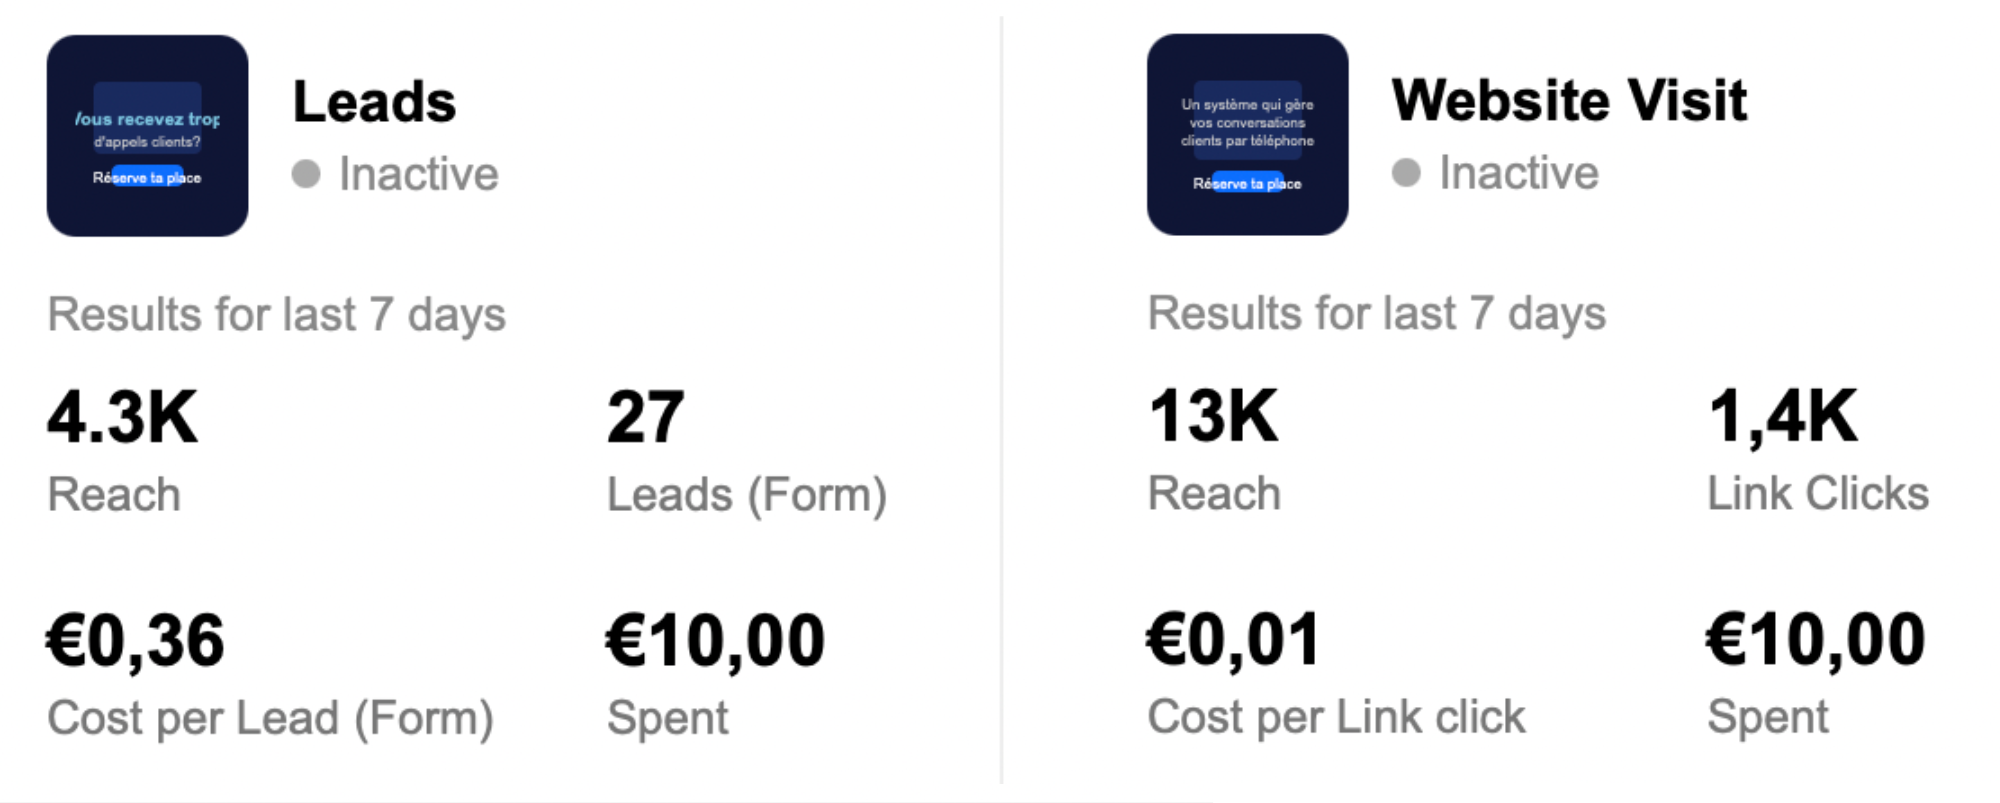
\includegraphics[width=0.78\textwidth]{figures/meta-ads-results.png}
    \caption{Résultats des campagnes Meta Ads --- Phase Muvaka (7 jours)}
    \label{fig:meta-ads-results}
\end{figure}

\textbf{Lecture analytique.} Le taux de clic de 10,9~\% (clics/\emph{reach}) sur la campagne \emph{Website Visit} dépasse de 7 à 20 fois les benchmarks B2B observés sur Meta Ads (0,5 -- 1,5~\%)~: c'est un signal de résonance forte du message auprès de l'audience ciblée. Le coût par lead de 0,36~\euro{} représente moins de 10~\% des moyennes B2B sectorielles (3 -- 15~\euro{}), indiquant une adéquation précise entre le ciblage et la douleur adressée. Ces résultats doivent être interprétés avec la prudence imposée par le budget limité et la durée courte de la campagne --- ils constituent néanmoins des signaux d'adéquation marché-message parmi les plus favorables qu'une phase exploratoire puisse produire à ce niveau de coût.

%%%%%%%%%%%%%%%%%%%%%%%%%%%%%%%%%%%%%%%%%%%%%%%%%%%%%%%%%%%%%%%%%%%%%%%%%%%
\subsection{Analyse des résultats du formulaire (22 répondants, e-commerçants actifs)}
\label{section2.4.3}
%%%%%%%%%%%%%%%%%%%%%%%%%%%%%%%%%%%%%%%%%%%%%%%%%%%%%%%%%%%%%%%%%%%%%%%%%%%

Le formulaire ciblait quatre dimensions~: profil du répondant, réalité du problème opérationnel, réceptivité à la solution et sensibilité prix.

\begin{table}[H]
\centering
\caption{Résultats du formulaire de recherche Muvaka --- 22 répondants}
\smallskip
\begin{tabular}{|p{2.8cm}|p{4.2cm}|p{4.8cm}|}
\hline
\textbf{Dimension} & \textbf{Résultat observé} & \textbf{Interprétation stratégique} \\
\hline
Ancienneté & 68,2~\% actifs depuis 3 ans ou plus & Marchands expérimentés~: ils connaissent le problème, ils ont déjà tout essayé \\
\hline
Volume appels/jour & 54,6~\% déclarent 6 appels ou plus & Charge opérationnelle récurrente, seuil de rentabilité de l'automatisation atteint \\
\hline
Gestion des appels & 52,4~\% par le gérant, 42,9~\% par un employé & Coût d'opportunité maximal~: ressources décisionnelles mobilisées sur du répétitif \\
\hline
Perte d'opportunités & \textbf{77,3~\% déclarent avoir perdu des ventes} & La friction opérationnelle se traduit directement en chiffre d'affaires perdu \\
\hline
Intérêt IA dialecte TN & 85~\% score 4 ou 5/5 & Réceptivité forte --- la barrière n'est pas culturelle mais technologique \\
\hline
Disposition à tester & \textbf{90,9~\% répondent Oui à un pilote} & Risque commercial d'acquisition quasi nul en phase de lancement \\
\hline
Sensibilité prix & 40,9~\% acceptent 50--150 DT/mois & Zone de pricing viable, cohérente avec le modèle SaaS projeté \\
\hline
\end{tabular}
\end{table}


Trois chiffres concentrent l'essentiel de la validation terrain. La figure~\ref{fig:kpi-muvaka} les isole pour en faire ressortir la force~: problème confirmé, solution désirée, adoption acquise.

\begin{figure}[H]
    \centering
    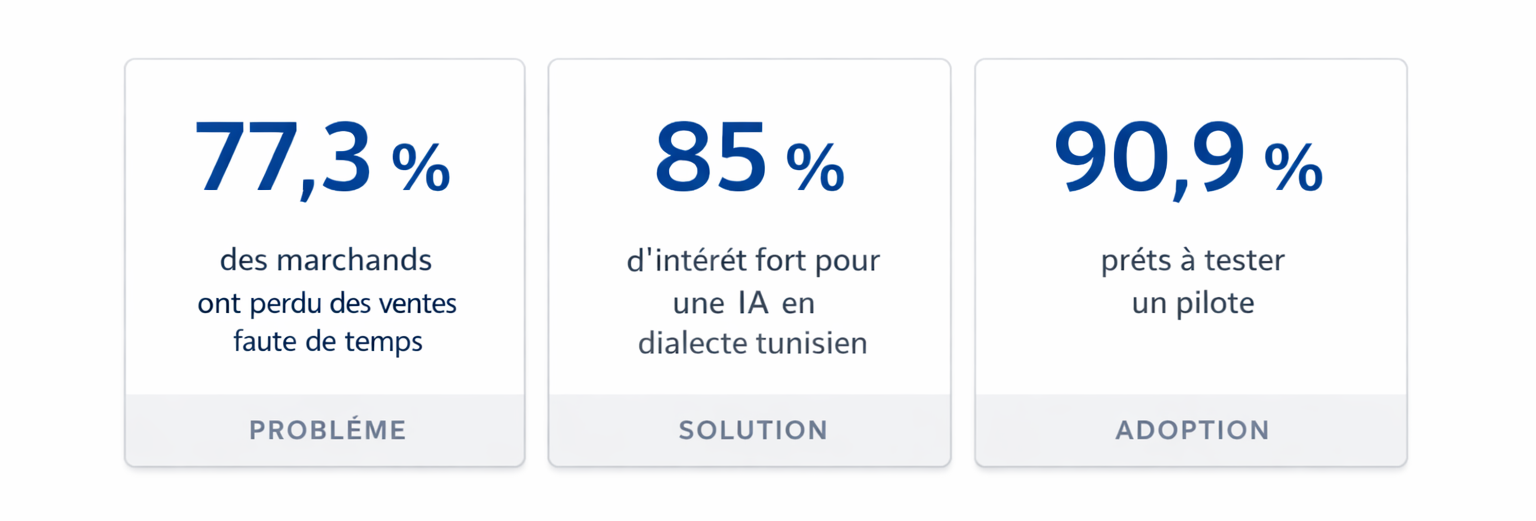
\includegraphics[width=0.95\textwidth]{figures/kpi-muvaka-triptyque.png}
    \caption{Triptyque de validation Muvaka --- Les trois signaux décisifs}
    \label{fig:kpi-muvaka}
\end{figure}

Le taux de 77,3~\% de marchands déclarant avoir perdu des ventes faute de temps transforme un problème d'efficacité en un \textbf{problème de chiffre d'affaires directement quantifiable} --- l'argument ROI le plus puissant disponible en démonstration B2B. Associé à 90,9~\% de disposition à tester un pilote, ce résultat révèle un marché non pas à convaincre, mais à équiper.

%%%%%%%%%%%%%%%%%%%%%%%%%%%%%%%%%%%%%%%%%%%%%%%%%%%%%%%%%%%%%%%%%%%%%%%%%%%
\subsection{Analyse des verbatims --- expression spontanée du problème}
\label{section2.4.4}
%%%%%%%%%%%%%%%%%%%%%%%%%%%%%%%%%%%%%%%%%%%%%%%%%%%%%%%%%%%%%%%%%%%%%%%%%%%

La question ouverte «~Quel est votre principal problème avec les appels clients~?~» (17 répondants) a généré des réponses spontanées en dialecte tunisien d'une clarté saisissante.

\begin{table}[H]
\centering
\caption{Verbatims --- expression spontanée du problème (dialecte tunisien)}
\smallskip
\begin{tabular}{|p{3.5cm}|p{3.5cm}|p{4cm}|}
\hline
\textbf{Verbatim (dialecte)} & \textbf{Traduction} & \textbf{Friction identifiée} \\
\hline
\og{}Ma yahezouch alik baad l confirmation\fg{} & Le client ne répond plus après confirmation & Annulation post-confirmation~: coût double \\
\hline
\og{}Tadhi3 wakt\fg{} & Perte de temps significative & Coût d'opportunité chronique \\
\hline
\og{}Totlob barcha marrat ou inajim yenssel ba3d\fg{} & Trop de tentatives sans résultat & Joignabilité faible, épuisement opérationnel \\
\hline
\og{}Ki manakhlatsh njawb, il annule mayhezesh\fg{} & Si on ne répond pas, la commande est annulée & Perte directe de CA par défaut de réactivité \\
\hline
\og{}Sa3t ma yefhemkch kol mara w kifeh\fg{} & Qualité variable de chaque échange & Absence de standardisation, risque image \\
\hline
\end{tabular}
\end{table}


Ces cinq verbatims couvrent l'intégralité du spectre de la friction~: non-joignabilité, perte de temps, annulation post-confirmation, perte de CA par défaut de réactivité, et variabilité qualitative. Leur expression spontanée en darija confirme que Vocallia doit parler la langue du problème --- littéralement. La maîtrise du dialecte n'est pas une fonctionnalité~: c'est la condition de l'adoption. Ces témoignages révèlent en creux une vérité plus large~: la question pour ces marchands n'est plus de savoir \emph{s'ils} automatiseront la confirmation, mais \emph{quand} --- et avec quel outil.

Au total, l'étude Muvaka valide simultanément les trois hypothèses fondamentales de tout modèle d'investissement \emph{early-stage}~: le problème est réel et douloureux~; la solution est désirée~; le prix est acceptable. L'étape suivante est leur confirmation à plus grande échelle --- mais la direction est établie avec un niveau de certitude suffisant pour déclencher l'exécution.

\medskip
La demande étant validée par le terrain, il reste à établir que l'espace concurrentiel est effectivement vide --- et à comprendre pourquoi il l'est.

%%%%%%%%%%%%%%%%%%%%%%%%%%%%%%%%%%%%%%%%%%%%%%%%%%%%%%%%%%%%%%%%%%%%%%%%%%%
\section{Analyse concurrentielle --- Benchmark local et international}
\label{section2.5}
%%%%%%%%%%%%%%%%%%%%%%%%%%%%%%%%%%%%%%%%%%%%%%%%%%%%%%%%%%%%%%%%%%%%%%%%%%%

L'analyse concurrentielle est conduite à deux niveaux~: le marché tunisien, pour cartographier les alternatives existantes et leurs limites~; le marché international, pour situer Vocallia face aux solutions d'IA vocale de référence mondiale.

%%%%%%%%%%%%%%%%%%%%%%%%%%%%%%%%%%%%%%%%%%%%%%%%%%%%%%%%%%%%%%%%%%%%%%%%%%%
\subsection{Alternatives disponibles sur le marché tunisien}
\label{section2.5.1}
%%%%%%%%%%%%%%%%%%%%%%%%%%%%%%%%%%%%%%%%%%%%%%%%%%%%%%%%%%%%%%%%%%%%%%%%%%%

Trois catégories de solutions existent sur le marché tunisien~: agents humains internes, centres d'appels externalisés, et outils de messagerie automatisée. \textbf{Aucun acteur ne propose à ce jour d'agent vocal IA en dialecte tunisien pour les e-commerçants.} Cette lacune reflète la complexité linguistique du darija et l'absence jusqu'ici d'une équipe locale capable de l'adresser techniquement.

\begin{table}[H]
\centering
\caption{Comparaison des alternatives sur le marché tunisien}
\smallskip
\begin{tabular}{|p{3cm}|l|l|l|l|}
\hline
\textbf{Critère} & \textbf{Agents internes} & \textbf{Call centers} & \textbf{Chatbots} & \textbf{Vocallia} \\
\hline
Appel vocal sortant & Oui & Oui (humain) & Non & Oui (IA) \\
\hline
Dialecte tunisien & Oui & Oui (humain) & Partiel & Oui (natif) \\
\hline
Scalabilité & Très limitée & Limitée & Élevée & Élevée \\
\hline
Coût / appel & Élevé & Élevé & Très faible & Faible \\
\hline
Traçabilité & Faible & Faible & Modérée & Élevée \\
\hline
Disponibilité 24h/24 & Non & Non & Oui & Oui \\
\hline
\end{tabular}
\end{table}


%%%%%%%%%%%%%%%%%%%%%%%%%%%%%%%%%%%%%%%%%%%%%%%%%%%%%%%%%%%%%%%%%%%%%%%%%%%
\subsection{Benchmark international --- solutions Voice AI globales}
\label{section2.5.2}
%%%%%%%%%%%%%%%%%%%%%%%%%%%%%%%%%%%%%%%%%%%%%%%%%%%%%%%%%%%%%%%%%%%%%%%%%%%

Les plateformes d'agents vocaux IA internationales --- Bland.ai, Vapi.ai, Retell, ElevenLabs --- ont émergé ces deux dernières années, portées par la démocratisation des API de langage et de synthèse vocale. Elles constituent la référence technologique mondiale, mais aucune n'adresse le marché tunisien.

\begin{table}[H]
\centering
\caption{Benchmark international --- solutions Voice AI globales}
\smallskip
\begin{tabular}{|p{2.8cm}|l|l|l|l|l|}
\hline
\textbf{Critère} & \textbf{Bland.ai} & \textbf{Vapi.ai} & \textbf{Retell} & \textbf{ElevenLabs} & \textbf{Vocallia} \\
\hline
Dialecte arabe TN & Non & Non & Non & Partiel & Oui \\
\hline
Code-switching AR/FR & Non & Non & Non & Non & Oui \\
\hline
Coût / appel 2 min & 0,18~\$ & 0,14~\$ & 0,14~\$ & 0,24~\$ & 0,10~\$ \\
\hline
Déploiement local & Non & Non & Non & Non & Prévu \\
\hline
Support MENA/TN & Non & Non & Non & Non & Oui \\
\hline
Pricing PME en DT & Non & Non & Non & Non & Oui \\
\hline
\end{tabular}
\end{table}


La figure~\ref{fig:radar-positionnement} traduit visuellement la dominance de Vocallia sur l'ensemble des critères pertinents pour le marché tunisien. Les acteurs internationaux ne sont pas des concurrents directs --- ils sont des fournisseurs de technologie générique incapables d'adresser la dimension linguistique, opérationnelle et économique du marché local sans un investissement dédié qu'aucun d'eux n'a engagé.

\begin{figure}[H]
    \centering
    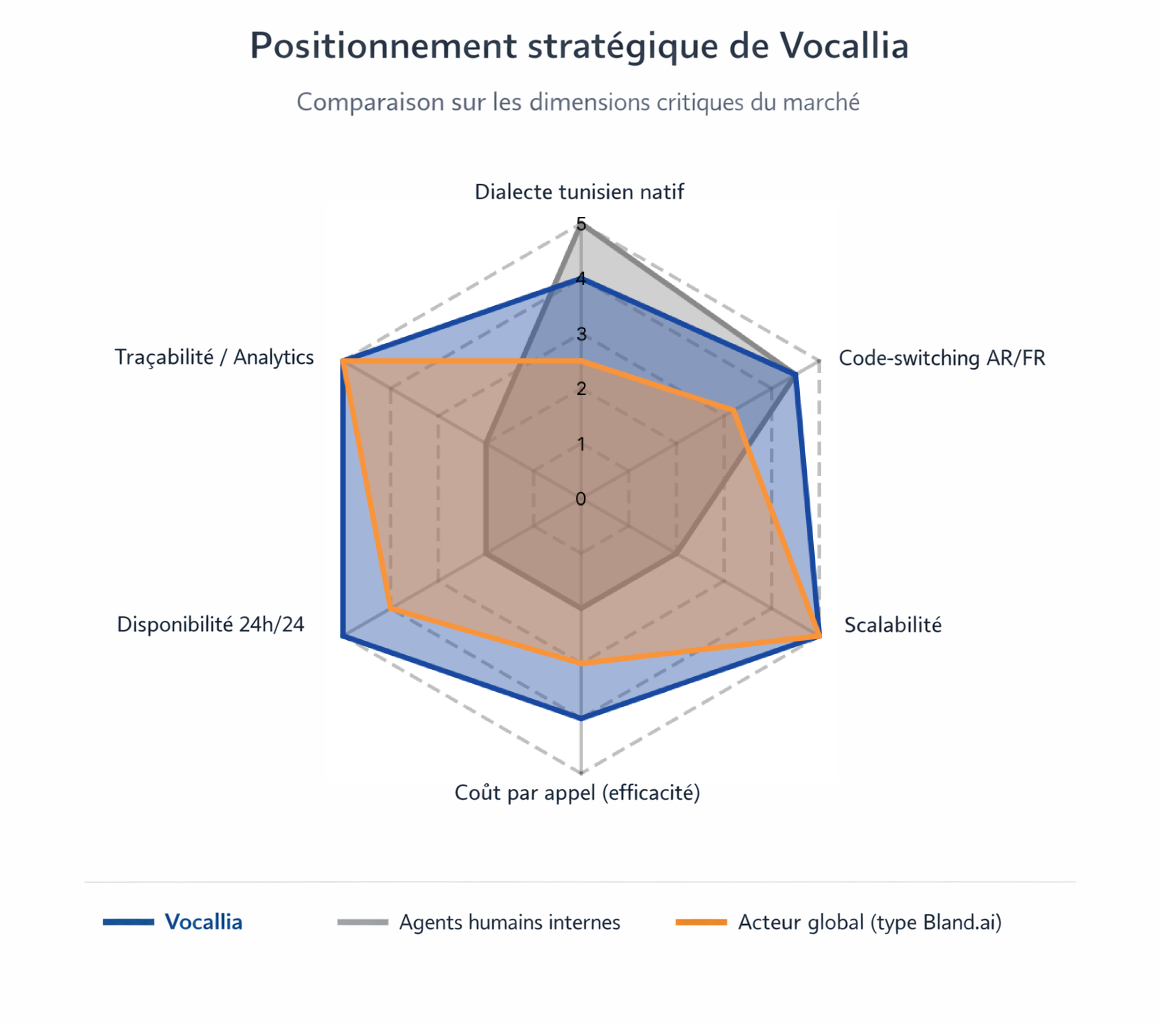
\includegraphics[width=0.75\textwidth]{figures/radar-positionnement-vocallia.png}
    \caption{Positionnement concurrentiel multidimensionnel --- Vocallia vs. alternatives}
    \label{fig:radar-positionnement}
\end{figure}

Le fossé concurrentiel qui en résulte repose sur quatre piliers auto-renforçants, dont le mécanisme central --- le \emph{flywheel} de données --- est représenté en figure~\ref{fig:flywheel-vocallia}.

\begin{figure}[H]
    \centering
    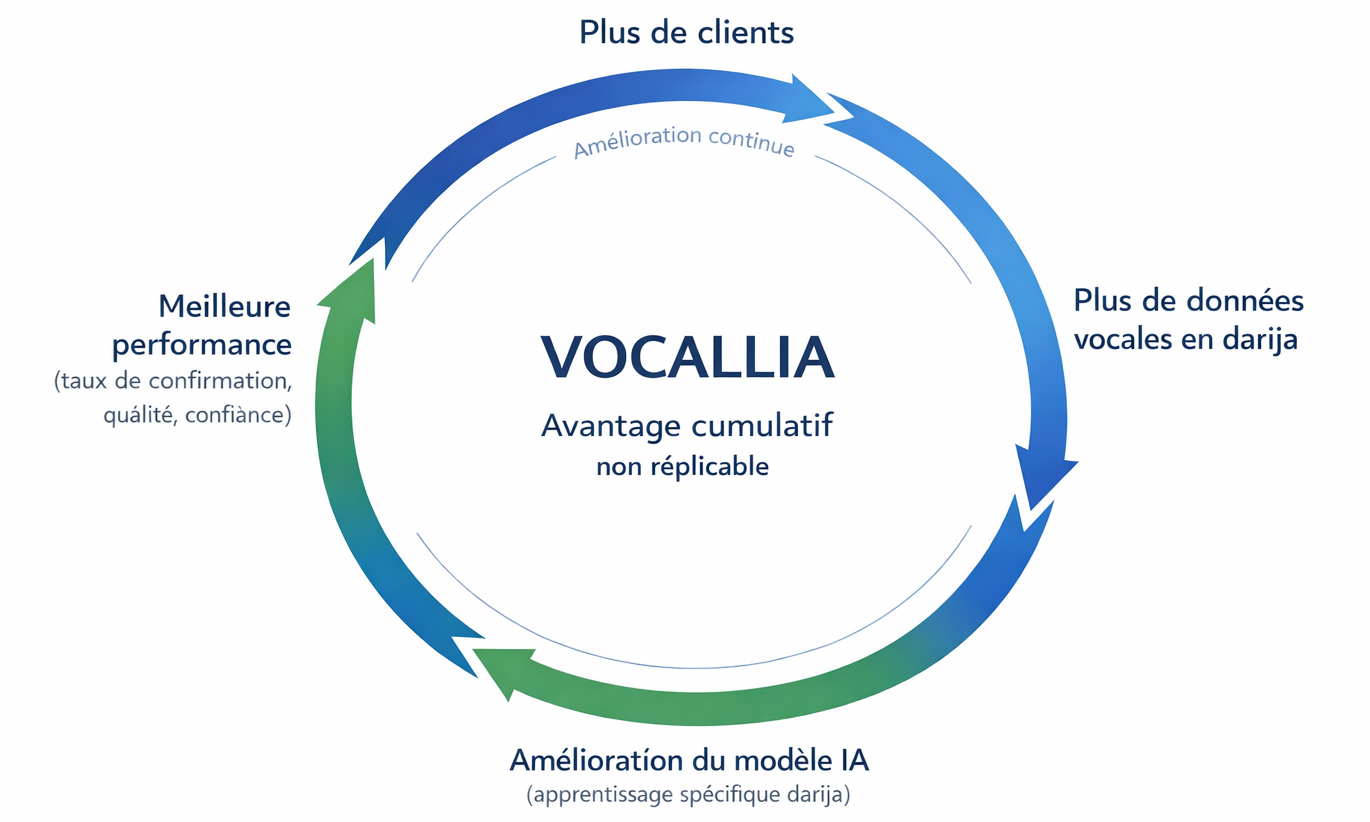
\includegraphics[width=0.68\textwidth]{figures/flywheel-vocallia.png}
    \caption{Mécanisme de \emph{flywheel} --- L'avantage concurrentiel auto-renforçant de Vocallia}
    \label{fig:flywheel-vocallia}
\end{figure}

\begin{tcolorbox}[colback=gray!8, colframe=gray!50, title=\textbf{Fossé concurrentiel de Vocallia --- Architecture du \emph{Moat}}, fonttitle=\bfseries]
Le fossé concurrentiel de Vocallia repose sur quatre piliers complémentaires et auto-renforçants, qui ensemble forment une position défendable sur un horizon de 3 à 5~ans.

La \textbf{barrière linguistique} constitue l'avantage immédiat~: le dialecte tunisien, non standardisé, à code-switching arabe/français dense, est une langue que les modèles globaux ne maîtrisent pas sans données locales. Cette maîtrise ne s'achète pas~: elle se construit par accumulation d'exemples réels et d'itérations sur le terrain.

Le \textbf{corpus de données propriétaires} génère un avantage croissant~: chaque appel traité enrichit un corpus exclusif et non reproductible. À 10\,000 appels, l'écart est significatif. À 100\,000 appels, il est infranchissable. Chaque point de précision gagné se traduit directement en livraisons échouées évitées --- et donc en valeur économique mesurable.

Le \textbf{mécanisme de \emph{flywheel}} (figure~\ref{fig:flywheel-vocallia}) produit un avantage exponentiel~: données $\rightarrow$ amélioration du modèle $\rightarrow$ meilleures performances $\rightarrow$ nouveaux clients $\rightarrow$ davantage de données.

Enfin, les \textbf{intégrations locales et \emph{switching costs}} assurent la rétention~: les intégrations avec les workflows tunisiens, combinées à la personnalisation des scripts, créent des coûts de changement significatifs et croissants. Chaque client intégré est un client structurellement fidélisé.

\medskip
\noindent Ensemble, ces quatre piliers positionnent Vocallia comme le seul acteur capable d'adresser simultanément la dimension linguistique, opérationnelle, économique et réglementaire du marché tunisien --- avantage compétitif défendable et auto-renforçant sur un horizon de trois à cinq ans.
\end{tcolorbox}

%%%%%%%%%%%%%%%%%%%%%%%%%%%%%%%%%%%%%%%%%%%%%%%%%%%%%%%%%%%%%%%%%%%%%%%%%%%
\section{Identification et cartographie des parties prenantes}
\label{section2.6}
%%%%%%%%%%%%%%%%%%%%%%%%%%%%%%%%%%%%%%%%%%%%%%%%%%%%%%%%%%%%%%%%%%%%%%%%%%%

La cartographie des parties prenantes identifie les acteurs qui conditionnent le développement de Vocallia, leurs attentes et la nature de leur influence sur la trajectoire du projet.

\begin{table}[H]
\centering
\caption{Cartographie des parties prenantes --- Vocallia}
\smallskip
\begin{tabular}{|p{2.5cm}|p{2cm}|p{4cm}|p{4cm}|}
\hline
\textbf{Partie prenante} & \textbf{Type} & \textbf{Attentes principales} & \textbf{Nature de l'influence} \\
\hline
E-commerçants (B2B) & Client direct & ROI mesurable, intégration fluide, prix accessible & \textbf{Déterminante}~: adoption = validation commerciale et génération de données \\
\hline
Clients finaux (acheteurs) & Utilisateur indirect & Appel naturel, bref, en dialecte local & Forte~: expérience négative = image dégradée pour le marchand partenaire \\
\hline
Providers API (OpenAI, ElevenLabs, Twilio) & Fournisseur & Volume d'appels, respect des CGU & Modérée~: contraintes tarifaires et quotas techniques \\
\hline
INPDP & Régulateur & Conformité loi 2004-63, licéité du traitement vocal & Modérée à élevée~: conditionne l'autorisation opérationnelle \\
\hline
Investisseurs / Startup Act & Financeur & Traction, croissance, équipe, défendabilité du modèle & \textbf{Élevée}~: conditionne le financement et la vitesse d'exécution \\
\hline
Équipe fondatrice & Interne & Vision, ressources, exécution & \textbf{Déterminante}~: la qualité d'exécution est le principal facteur de succès \\
\hline
\end{tabular}
\end{table}

Deux parties prenantes conditionnent la trajectoire à court terme de manière asymétrique. Les e-commerçants clients sont le moteur primaire~: chaque client acquis valide le modèle, génère des données propriétaires et produit un revenu récurrent. L'INPDP constitue le verrou réglementaire~: l'engager proactivement avant le déploiement commercial transforme une contrainte potentielle en signal de crédibilité vis-à-vis des investisseurs et des clients institutionnels. La priorité opérationnelle des six premiers mois est ainsi clairement établie~: acquérir les premiers clients pilotes et obtenir la validation réglementaire --- dans cet ordre de levier, mais en parallèle d'exécution.

%%%%%%%%%%%%%%%%%%%%%%%%%%%%%%%%%%%%%%%%%%%%%%%%%%%%%%%%%%%%%%%%%%%%%%%%%%%
\section{Carte d'empathie --- Profil du client cible}
\label{section2.7}
%%%%%%%%%%%%%%%%%%%%%%%%%%%%%%%%%%%%%%%%%%%%%%%%%%%%%%%%%%%%%%%%%%%%%%%%%%%

La carte d'empathie (Osterwalder \& Pigneur, 2010~; Dave Gray, 2010) permet de dépasser la description fonctionnelle du client pour appréhender sa réalité vécue. Pour Vocallia, le profil cible est le gérant ou responsable opérationnel d'une boutique e-commerce tunisienne traitant 10 à 50 commandes par jour~: un entrepreneur dont la croissance est freinée non par l'absence de demande, mais par une incapacité opérationnelle à traiter le volume d'interactions clients avec les ressources disponibles.

\begin{figure}[H]
    \centering
    
\includegraphics[width=\textwidth]{carte-empathie-vocallia.png}
    \caption{Carte d'empathie --- Profil du client cible Vocallia}
    \label{fig:empathie-vocallia}
\end{figure}

\textit{Source~: Inspiré de Dave Gray, Empathy Map Canvas (2010) --- enrichi des données de l'étude exploratoire Muvaka (collecte avril 2025).}

Ce profil éclaire un impératif stratégique fondamental~: le client cible ne cherche pas une solution d'IA --- il cherche à récupérer du temps, à ne plus perdre de ventes et à sortir du cycle épuisant des appels répétitifs. L'argument de vente de Vocallia n'est pas technologique --- il est économique et humain~: «~Combien de ventes avez-vous perdues ce mois-ci par manque de temps pour rappeler~?~» La réponse à cette question, documentée par les données Muvaka (77,3~\% de marchands concernés), est le meilleur commercial que Vocallia puisse avoir.

%%%%%%%%%%%%%%%%%%%%%%%%%%%%%%%%%%%%%%%%%%%%%%%%%%%%%%%%%%%%%%%%%%%%%%%%%%%
\section{Conclusion}
\label{conclusion2}
%%%%%%%%%%%%%%%%%%%%%%%%%%%%%%%%%%%%%%%%%%%%%%%%%%%%%%%%%%%%%%%%%%%%%%%%%%%

L'analyse de marché conduite dans ce chapitre établit quatre conclusions qui fondent la thèse d'investissement de Vocallia.

\textbf{Le marché est captif.} Avec 84~\% des transactions réglées en \emph{cash on delivery} et une croissance sectorielle de 41,6~\%, la confirmation téléphonique n'est pas un choix --- c'est une obligation opérationnelle dont l'intensité croît avec le volume. Même pour un petit marchand traitant 10 à 15 commandes par jour, le coût cumulé des retours et de la gestion manuelle des appels représente entre 700 et 1\,400~DT par mois (figure~\ref{fig:cout-commande-non-confirmee}) --- charge significative pour une PME aux marges étroites, et suffisante pour justifier le recours à l'automatisation.

\textbf{La demande est validée.} 77,3~\% des marchands interrogés associent le problème à une perte directe de chiffre d'affaires, 85~\% expriment un intérêt fort pour une IA en dialecte tunisien, 90,9~\% acceptent un pilote (figure~\ref{fig:kpi-muvaka}). Signal directionnel suffisant pour déclencher l'exécution.

\textbf{L'espace concurrentiel est vide --- et temporairement.} Aucune solution ne combine voix IA, darija natif, code-switching et pricing PME (figure~\ref{fig:radar-positionnement}). Le fossé de Vocallia --- données propriétaires, \emph{flywheel}, \emph{switching costs} --- se compose avec le temps. Mais il ne se construit que si la position est occupée maintenant.

\textbf{La fenêtre est ouverte --- mais bornée.} IA vocale mature, coûts API décroissants, Startup Act mobilisable, marché vierge. Dans 18 à 36~mois, ces conditions auront changé (figure~\ref{fig:timeline-fenetre}).

\begin{figure}[H]
    \centering
    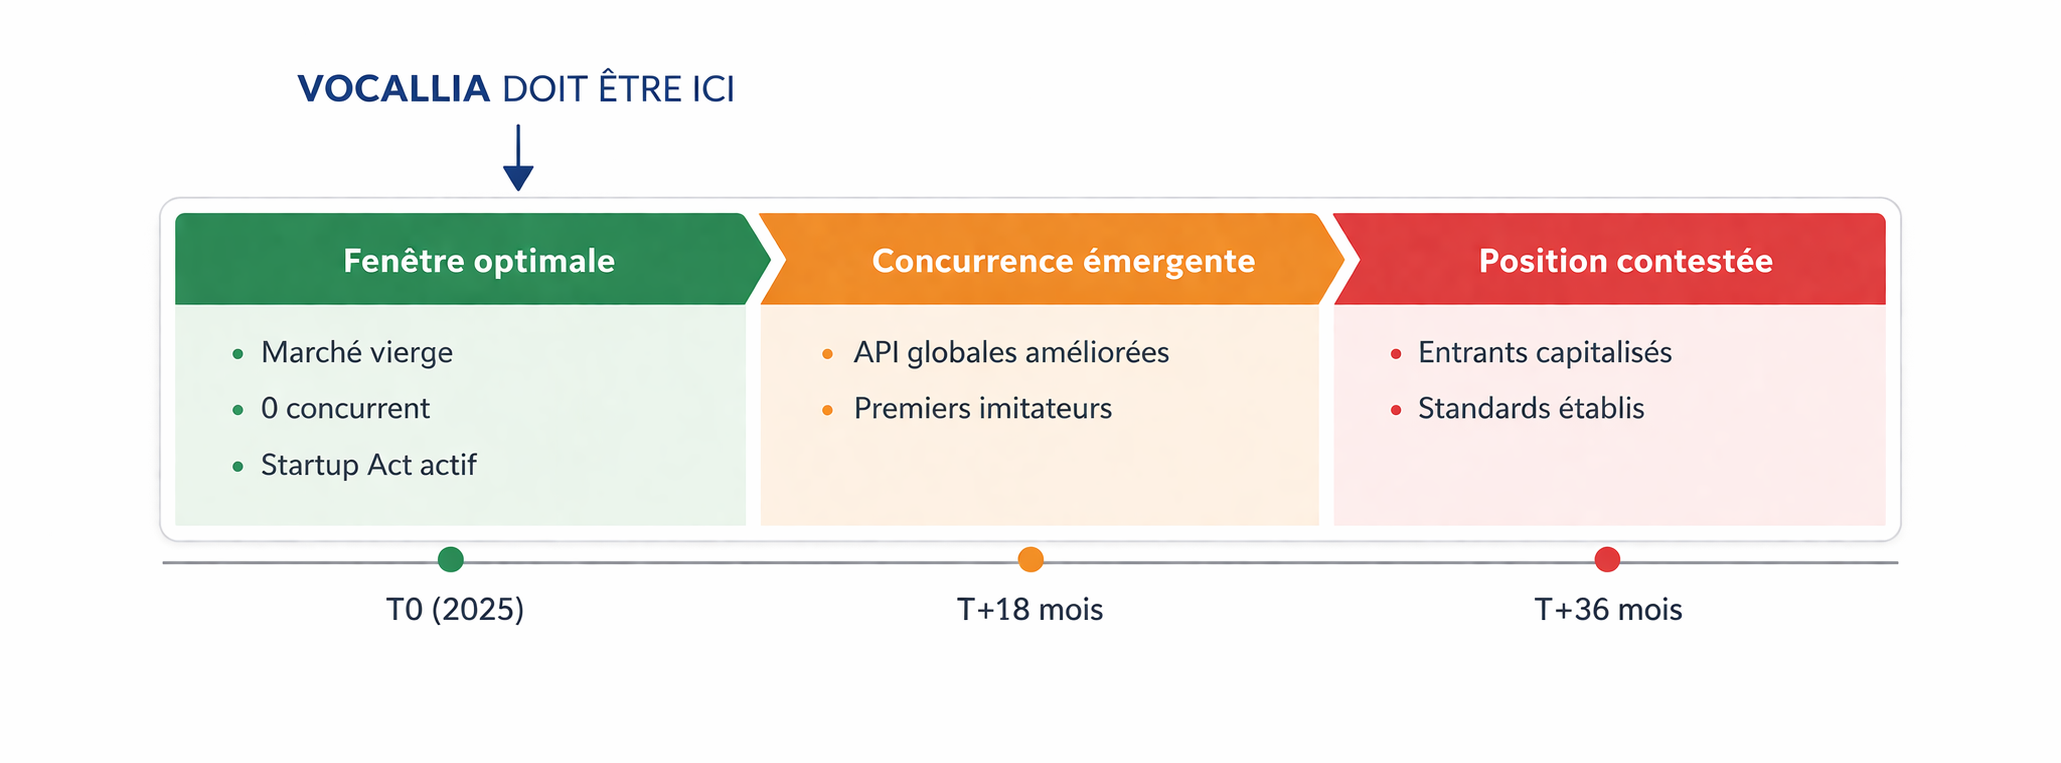
\includegraphics[width=0.95\textwidth]{figures/timeline-fenetre-execution.png}
    \caption{Fenêtre d'exécution de Vocallia --- Urgence temporelle et dynamique concurrentielle}
    \label{fig:timeline-fenetre}
\end{figure}

Vocallia ne se positionne pas comme un outil ponctuel, mais comme la première brique d'une infrastructure conversationnelle en dialecte tunisien --- un actif dont la valeur croît avec chaque interaction, chaque client, chaque verticale. Le marché ne demande pas si cette transition aura lieu~: il demande qui l'opérera en premier.

\begin{tcolorbox}[colback=gray!8, colframe=gray!50, title=\textbf{Thèse d'investissement}, fonttitle=\bfseries]
\begin{center}
\emph{Inefficience non optionnelle. Marché captif en croissance. Espace concurrentiel vide. Fossé défendable qui se renforce par l'usage. La question n'est pas de savoir si le e-commerce tunisien automatisera la confirmation vocale --- mais si Vocallia sera celui qui imposera le standard. La fenêtre est ouverte. Elle ne le restera pas.}
\end{center}
\end{tcolorbox}

\begin{quote}
\textit{Le chapitre suivant traduit ces fondations analytiques en stratégie commerciale opérationnelle~: segmentation, ciblage, proposition de valeur (Value Proposition Canvas), architecture de pricing et modèle économique SaaS --- en mobilisant les outils de la finance entrepreneuriale pour démontrer la viabilité et le potentiel de Vocallia à l'horizon trois ans.}
\end{quote}